\begin{figure}[htbp]
    \centering
    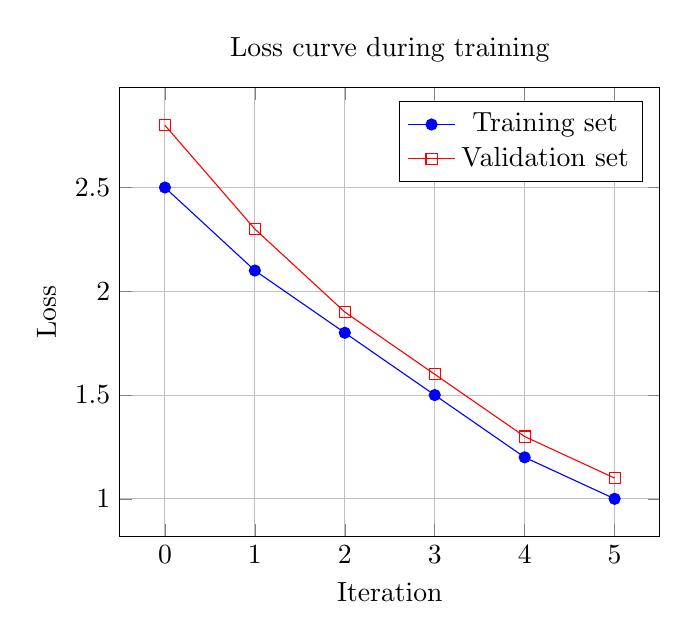
\begin{tikzpicture}
        \begin{axis}[
            xlabel={Iteration},
            ylabel={Loss},
            title={Loss curve during training},
            legend pos=north east,
            grid=major
        ]
        \addplot[color=blue,mark=*] coordinates {
            (0,2.5)
            (1,2.1)
            (2,1.8)
            (3,1.5)
            (4,1.2)
            (5,1.0)
        };
        \addplot[color=red,mark=square] coordinates {
            (0,2.8)
            (1,2.3)
            (2,1.9)
            (3,1.6)
            (4,1.3)
            (5,1.1)
        };
        \legend{Training set, Validation set}
        \end{axis}
    \end{tikzpicture}
    \caption{Example figure: Loss curve during training}
    \label{fig:loss-curve}
\end{figure} 